\section{Understanding how the Radon transform is performed}
With the theory in place, we can now move on and look at some more practical applications of the Radon transform. In python we can use the \textit{skimage} library to perform the Radon transform on images. In \autoref{shepp} we see the Shepp-Logan phantom which is a common test image. It is composed of several ovals with varying uniform intensity. The result of taking the Radon transform of this image can be seen in \autoref{sheppSinoHighRes}. The result is at first glance hard to interpret, as it would seem to be a lot of sinus waves laid on top of each other, and thus we will begin by analysing some simpler shapes and their sinograms, and then return to the Shepp-Logan image when we have a greater understanding.\\
\begin{figure}
	\centering
	\begin{subfigure}{0.48\linewidth}
		\centering
		
\includegraphics[width=\linewidth]{Materials/sheppLogan}
		\caption{The Shepp-Logan phantom.\newline\newline}
		\label{shepp}
	\end{subfigure}
	\hfill
	\begin{subfigure}{0.48\linewidth}
			\centering
			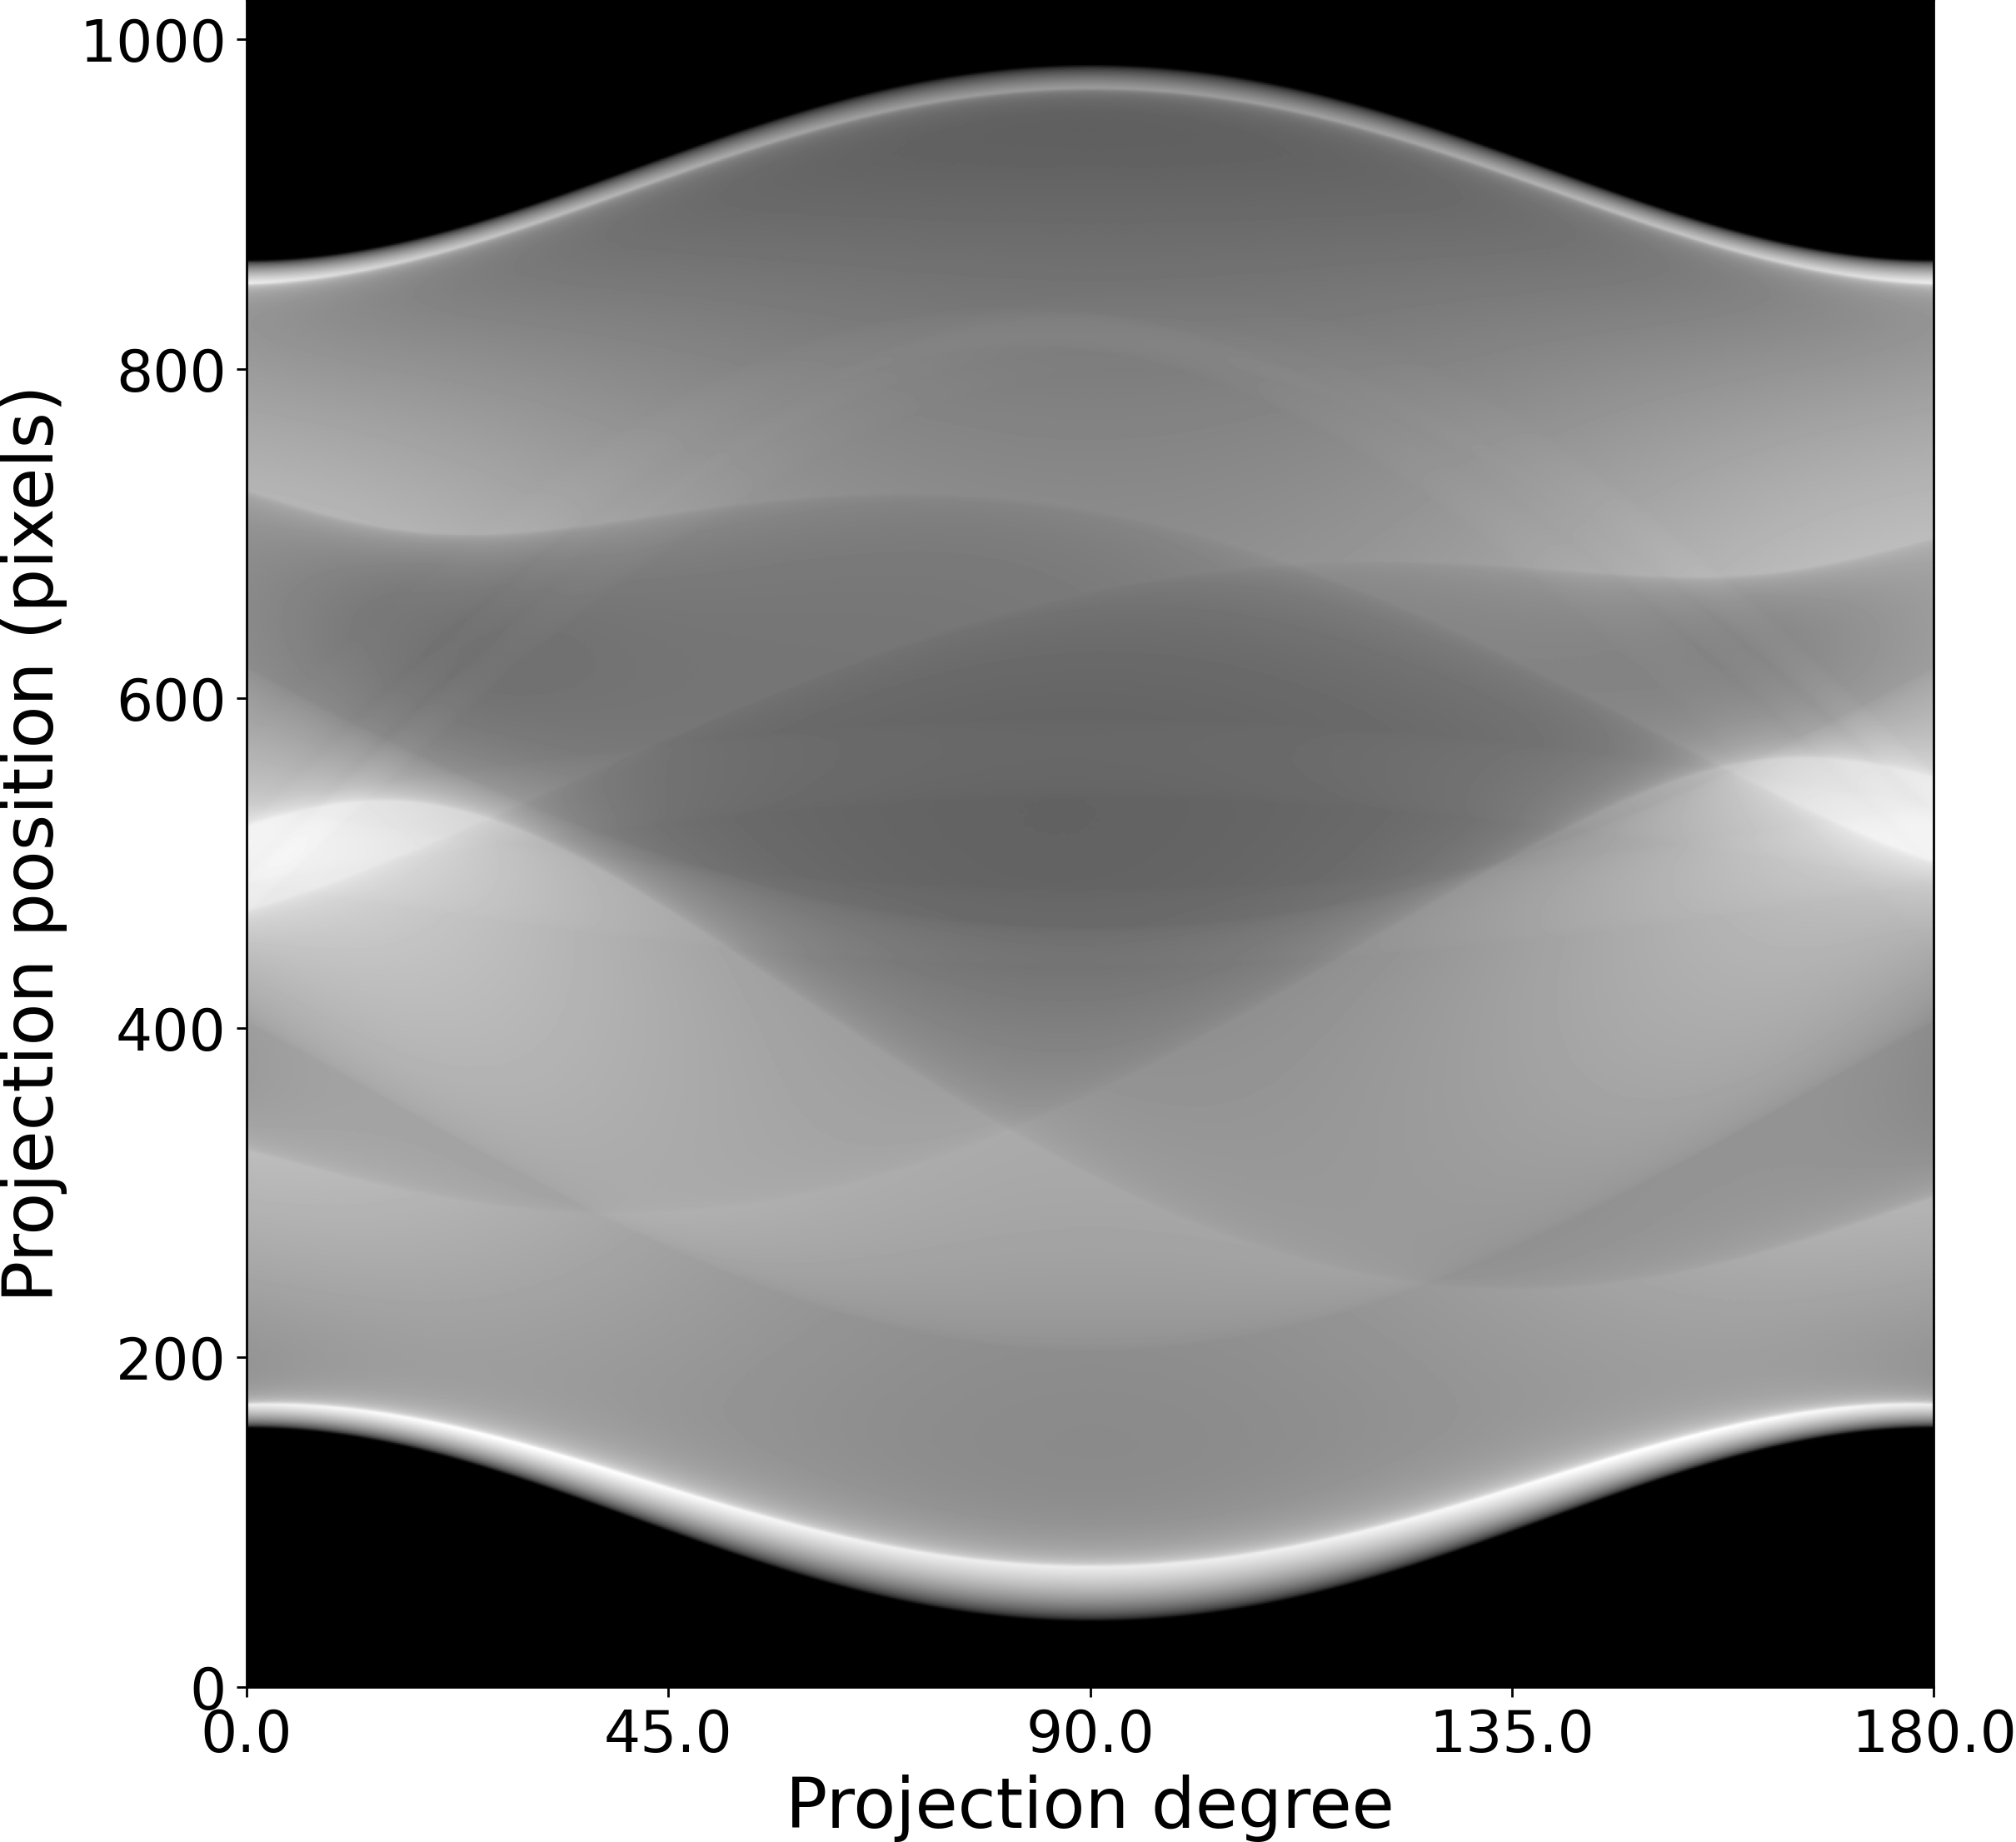
\includegraphics[width=\linewidth]{Materials/sheppLoganHighRes}
			\caption{Sinogram of The Shepp-Logan phantom taken with 1024 angles between 0 and 180 degrees.}
			\label{sheppSinoHighRes}
	\end{subfigure}
	\caption{The Shepp-Logan phantom along its sinogram computed over 180 degrees.}
\end{figure}
\begin{figure}
	\centering
	\begin{subfigure}{0.48\linewidth}
		\centering
		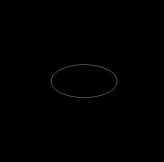
\includegraphics[width=\linewidth]{Materials/hEllipse}
		\caption{A vertical ellipse.\newline\newline}
		\label{hEllipse}
	\end{subfigure}
	\hfill
	\begin{subfigure}{0.48\linewidth}
		\centering
		
\includegraphics[height=1.5\linewidth]{Materials/hEllipseSino}
		\caption{Sinogram of a vertical ellipse taken with 180 angles between 0 and 180 degrees.}
		\label{hEllipseSino}
	\end{subfigure}
	\caption{A vertical ellipse and its sinogram.}
\end{figure}
In \autoref{hEllipse} we have drawn a simple vertical ellipse. Taking its sinogram we get the hourglass-shape seen in \autoref{hEllipseSino}. Thinking back to the theory, the sinograms are composed of several projections of the original object taken from several angles. In \autoref{hEllipseSino} we see the sinogram begins with a wide shape which then gets more narrow before it gets wide again. Based on these observations we can conclude the radon transform is initialized from either the top or the bottom of the original image.\\
\begin{figure}
	\centering
	\begin{subfigure}{0.48\linewidth}
		\centering
		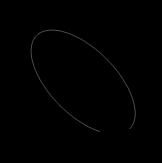
\includegraphics[width=\linewidth]{Materials/tEllipse}
		\caption{A slightly tilted ellipse.\newline\newline}
		\label{tEllipse}
	\end{subfigure}
	\hfill
	\begin{subfigure}{0.48\linewidth}
		\centering
		
\includegraphics[height=1.5\linewidth]{Materials/tEllipseSino}
		\caption{Sinogram of a slightly tilted ellipse taken with 180 angles between 0 and 180 degrees.}
		\label{tEllipseSino}
	\end{subfigure}
	\caption{A tilted ellipse and its sinogram.}
\end{figure}
In \autoref{tEllipse} we have tilted the ellipse slightly and in \autoref{tEllipseSino} we have its sinogram. We here see a shift in the narrow part as it now lies more to the left in the sinogram. This observation tells us we move in a counter clockwise motion around the original image when we do the Radon transform, as the narrow part of the ellipse is encountered first when starting either from the top or bottom and then moving counter clockwise around it.\\
As we now know we either start from the top or the bottom of the original image, and we move counter clockwise around it, we can now return to the sinogram of the Shepp-Logan image in \autoref{sheppSinoHighRes}. We note this sinogram is considerably more square than the other sinograms. This is due to the more angles used to obtain the sinogram. In the ellipses 180 angles between 0 and 180 degrees are used. This means each pixel column corresponds to a 1 degree turn. In the Shepp-Logan sinogram 1024 angles are used between 0 and 180 degrees. This means each pixel row is less than a 1 degree turn, however, we still begin at 0 degrees and end at 180 degrees, so end points of the images have the same relative meaning. Now looking at the middle part the of \autoref{sheppSinoHighRes} we see two darker shades, one being narrow and growing wider while moving from the top to the bottom, and one starting wide and growing narrow while moving from the bottom to the top. These two shades are the two big black ellipses in the middle of the Shepp-Logan phantom (\autoref{shepp}). We see this mainly because these are the darkest parts of the Shepp-Logan phantom, and so they will contribute with a low to no response in the sinogram, but we can also see based on our previous observations they behave as expected, as we begin the sinogram from either the top or bottom of the original image and move counter clockwise around it. As the two ellipses are slightly tilted to the opposite directions, we can actually determine that the sinogram is begun from the bottom, as the bigger of the dark shades in the sinogram begins in the top (left in the projection) in the sinogram and ends at the bottom (to the right in the projection). Had the Radon transform been begun from the top, we would have had seen the opposite.\\
But why have we chosen to only show 180 degrees? In \autoref{shepp360} we see a sinogram of the Shepp-Logan image taken from 1024 angles between 0 and 360 degrees. We here see a strong similarity to the 180 degrees sinogram in \autoref{sheppHighRes}, in fact, the first half (the first 180 degrees) is the same and the second is simply the first half mirrored. This also intuitively makes sense as the line integrals measure the intensities in the image 'the whole way through', and so, taking the sinogram from 180 degrees to 360 degrees gives the same response as from 0 to 180 degrees, simply mirrored in the \textit{x-axis}.
\begin{figure}
	\centering
	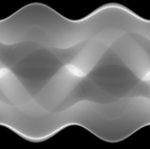
\includegraphics[width=0.5\linewidth]{Materials/shepp360}
	\caption{Sinogram of the Shepp-Logan image with 1024 angles between 0 and 360 degrees.}
	\label{shepp360}
\end{figure}